\documentclass[11pt,reqno]{beamer}
\usepackage[utf8x]{inputenc}
\usetheme{Dresden}
\usecolortheme{beaver}
\usepackage{amsmath}
\usepackage{amsfonts}
\usepackage{graphicx}

\setbeamertemplate{navigation symbols}{} 
\title{Bond Graph Clinic: Part 1}
\author{Peter Cudmore}

\institute{Systems Biology Lab, The University of Melbourne}

\newcommand{\D}[2]{\frac{\mathrm{d} #1}{\mathrm{d} #2}}
\newcommand{\e}{\mathrm{e}}
\newcommand{\I}{\mathrm{i}}
\renewcommand{\mod}[1]{\left|#1\right|}
\newcommand{\DD}[2]{\frac{\mathrm{d}^2 #1}{\mathrm{d} #2^2}}
\newcommand{\bigO}[1]{\text{O}\left(#1\right)}
\renewcommand{\P}[2]{\frac{\partial #1}{\partial #2}}
\renewcommand{\Re}{\operatorname{Re}}
\renewcommand{\Im}{\operatorname{Im}}
\newcommand{\EX}{\mathbb{E}}
\newcommand{\df}[1]{\mspace{2mu}  \mathrm{d}#1}
\newcommand{\reals}{\mathbb{R}}
\newcommand{\complex}{\mathbb{C}}
\newcommand{\conj}[1]{\overline{#1}}

\begin{document}
	\begin{frame}
	\titlepage
	\addtocounter{framenumber}{-1} 
\end{frame}
\begin{frame}
\tableofcontents[hideallsubsections]
\end{frame}
\section{Meta-modelling}
\subsection{Domain Specific Languages}
\begin{frame}
\frametitle{Assertions}
I hope to convince you that:
\begin{itemize}
	\item Bond Graphs are a general purpose modelling language for energetic systems.
	\item Bond Graphs (or something equivalent) emerge naturally from modelling energy distribution networks.
	\item Bond Graphs are a meta-modelling~\cite{gaw96} tool, and hence most powerful when considering multiple physical domains.
\end{itemize}
\end{frame}
\begin{frame}
\frametitle{Domain Specific Language}
Domain-specific languages (DSL) are computer (programming, scripting or mark-up) languages specific to a particular application domain.\\
\vspace{20pt}

Examples include: 
\begin{itemize}
	\item \emph{CellML} and \emph{SBML}
	\item \emph{Matlab}'s scripting language
	\item \emph{VHDL} or \emph{Verilog} (for hardware design)
	\item \LaTeX
\end{itemize}
\end{frame}
\begin{frame}
\frametitle{General Purpose Language}
In contrast, general-purpose languages are designed to be applicable in a wide variety of domains
\vspace{20pt}

Examples include: 
\begin{itemize}
	\item Assembly, C, C++
	\item Python
	\item XML, json
	\item ASCII  
\end{itemize}
\end{frame}

\subsection{Modelling Languages in Science and Engineering}
\begin{frame}
\frametitle{DSL's are not unique to software development.}
Graphical DSL's can be found in the natural sciences:
\begin{itemize}
	\item Feynman diagrams,
	\item Circuit schematics,
	\item Chemical reaction notation,
	\item Gene regulatory network diagrams,
\end{itemize}

Here we're focussing on dynamic systems.\\

\end{frame}

\begin{frame}
\frametitle{Example: Schematic}
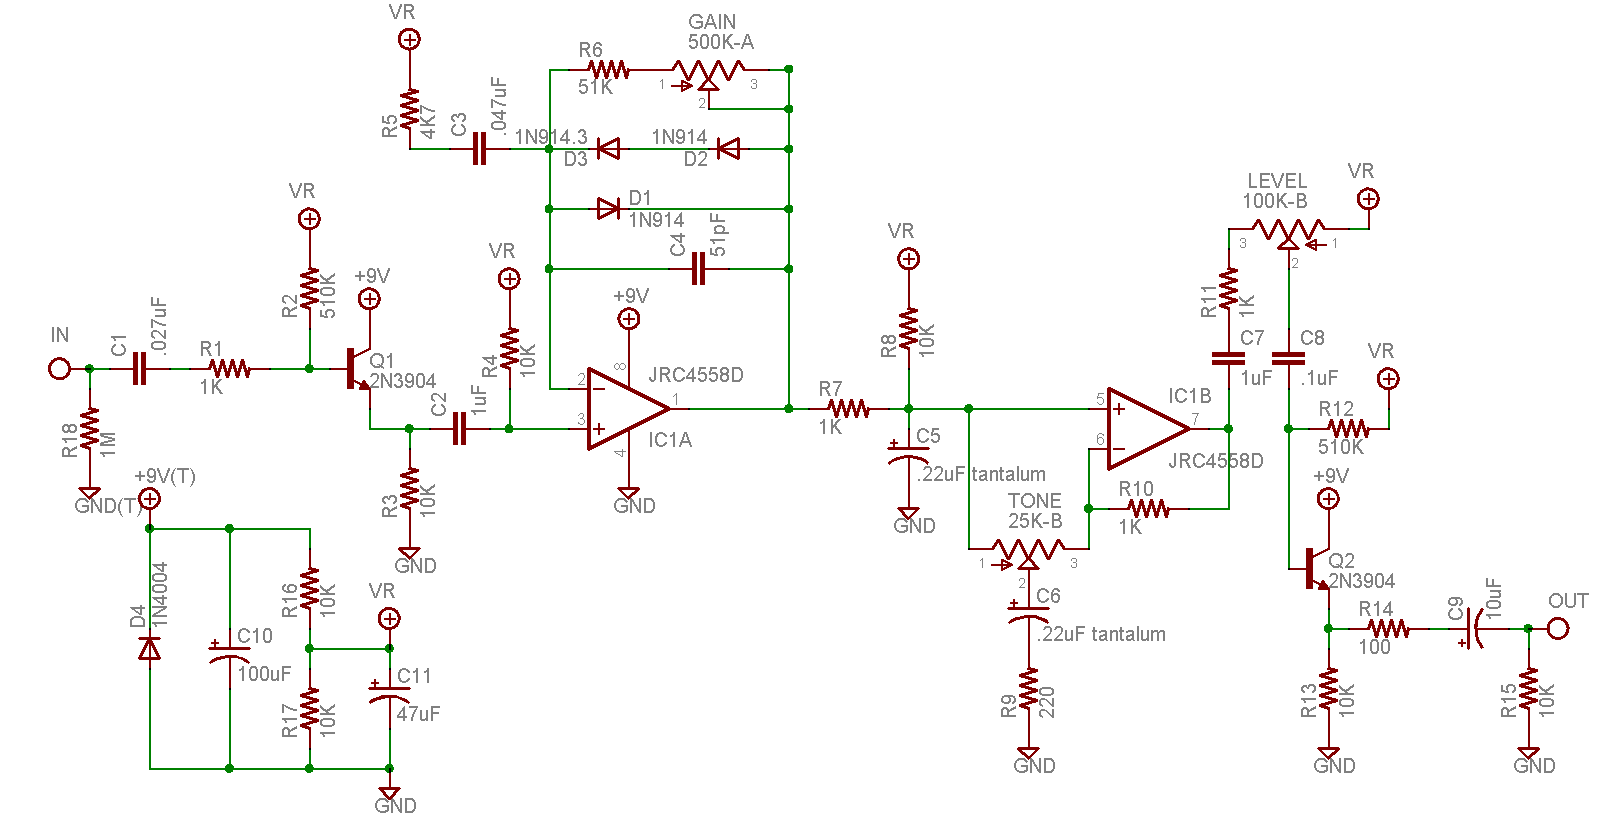
\includegraphics[width=\linewidth]{images/ts808.png}
\end{frame}
\begin{frame}
\frametitle{Example: CRN}
\begin{figure}
\centering 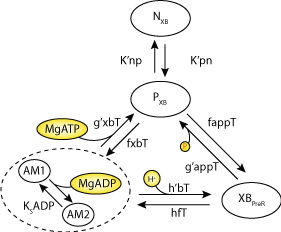
\includegraphics[height=4.5cm]{images/tran_2009.png}
\caption{Tran. \emph{et al.} \cite{Tran2009} }
\end{figure}
\end{frame}

\begin{frame}
\frametitle{General Purpose Modelling}
\begin{center}
\only{How to represent systems across multiple domains?}<1>
\only{
If physics and mathematics are the `machine language'\\ 
of physical systems modelling,
\vspace{20pt}

What's the equivalent of C?}<2>
\only{Bond Graphs}<3>
\only{
\vspace{2cm}

Bond Graphs*
\vspace{2cm}

\small{*Conditions Apply}}<4>
\end{center}
\end{frame}
\section{Bond Graphs}
\subsection{Structure}
\begin{frame}
\frametitle{Law of Conservation of Energy}
\begin{quotation}
There is a fact, or if you wish, a law, governing all natural phenomena that are known to date. There is no known exception to this law—it is exact so far as we know. The law is called the conservation of energy.
\end{quotation}

- Richard Feynman, 1961~\cite{Feynman1961}.
\end{frame}
\begin{frame}
\frametitle{Core Modelling Assumptions}
A general purpose physical modelling language must
\begin{itemize}
	\item use energy as the core currency.
	\item decompose a physical system into functionally discrete subsystems.
	\item describe the transfer of energy between subsystems.
\end{itemize}
\vspace{1cm}
These assumptions imply a network structure!

\end{frame}
\begin{frame}
\frametitle{Implied Network Structure}
\begin{figure}
	\centering
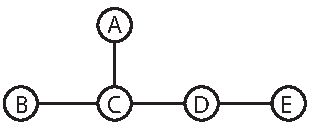
\includegraphics{images/network_1.pdf}
\caption{An Energy Network}
\end{figure}
Nodes represent energetic subsystems.

\vspace{5pt}

Edges represent transfer of energy between subsystems.
\end{frame}

\begin{frame}
\frametitle{Open Systems}
\begin{figure}
\centering
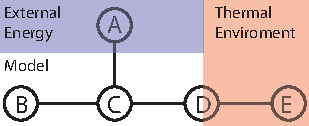
\includegraphics{images/network_2.pdf}
\end{figure}
\centering
is modelled as
\begin{figure}
	\centering
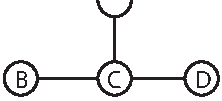
\includegraphics{images/network_2a.pdf}
\end{figure}
\end{frame}
\subsection{Energy \& Power}
\begin{frame}
\frametitle{A brief aside: Classical Mechanics}
\emph{Energy} is formally defined as the temporally invariant quantity of a closed system.\\
\vspace{12pt}

Energy comes in two forms, \emph{Potential Energy} and \emph{Kinetic Energy}.\\
\vspace{12pt}
\only{
\emph{Potential Energy} fundamentally depends on something like position $q$. Examples Include;
\begin{itemize}
	\item Gravitational potential energy $V(q_1,q_2) \propto -\frac{1}{|q_1-q_2}$, where $q_1,q_2$ are the spatial location of a point-masses.
	\item Elastic potential energy $V = \frac{1}{2}kq^2$ where $q$ is the displacement from equilibrium of a spring.
\end{itemize}}<2>
\only{
\emph{Kinetic Energy} fundamentally depends on motion. \\
The most common example is the newtonian kinetic energy of a mass $m$ in motion
$T = \frac{1}{2m}p^2$, where $p$ is the momentum of the moving object.}<3>
\end{frame}
\begin{frame}
\frametitle{A brief aside: Hamiltonian Mechanics}
In a closed system, the total energy $T+V$ is conserved.\\
Hence, we can define a energy function (called a Hamiltonian) $H:X\times X \rightarrow \mathbb{R}$ satisfying
\[
H(q,p) = T(p) + V(q) \implies \D{H}{t} = \P{H}{p}\dot{p} + \P{H}{q}\dot{q} = 0.
\]
We can easily recover Hamiltons equations:
\[
e = \dot{p} = -\D{H}{q}(q,p) ,\qquad f = \dot{q} = \D{H}{p}(q,p)
\]
The derivatives $e, f$ are \emph{effort} and \emph{flow} variables!
\end{frame}
\begin{frame}
\frametitle{Phase Space and State Space}
Notice
\begin{itemize}
	\item $H(q,p) =T(p) + V(q)$ has units of energy.
	\item $\D{H}{t}(q,p)$ and hence $\dot{p}\dot{q} = ef$  has units of power (rate of change of energy).
\end{itemize}
\emph{Power can always be factorised into a pair $P = ef$.} \\
\vspace{10pt}
For any subsystem, the energy should always satisfy
\[
\D{E}{t} = \D{H(q,p)}{t}  + D(q,\dot{q}) + P_\text{in} = 0 = \Phi(q,p, e_\text{in},f_\text{in})
\]
$\Phi$ is called the \emph{constitutive relation}. ($D$ is dissipation)
\end{frame}
\begin{frame}
\frametitle{Domain Specific Power}
{\tiny
\begin{tabular}{p{1.5cm} | p{1.75cm} | p{1.75cm} |p{1.75cm} | p{1.75cm}|}
Domain & $q$ & $f$ & $p$ & $e$\\
\hline
Translational Mechanics & position & velocity & momentum & force\\
\hline \\
Rotational Mechanics & angle & angular velocity & angular momentum & torque\\
\hline \\
Electronics & charge  & current & flux linkage & voltage\\
\hline \\
Hydraulics & volume & flow & pressure momentum & pressure\\
\hline \\
Thermodynamics & entropy & entropy flow & temperature momentum & temperature\\
\hline \\
Chemistry & moles & molar flow& chemical momentum & chemical potential\\
\hline 
\end{tabular}}
\end{frame}
\begin{frame}
\frametitle{Network Structure with 2-variable Edges}
System is represented by
\begin{figure}
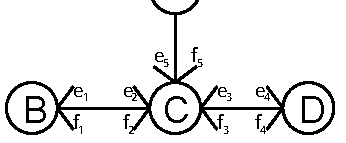
\includegraphics{images/portbondgraph.pdf}
\end{figure}
with the energetic behaviour of the $B$ subsystem is specified by
$\Phi_B(p_B,q_B,e_1,f_1)= 0$. Similarly for the $C$ and $D$ subsystems.
\end{frame}
\begin{frame}
\frametitle{Directed Network Structure}
\only<1>{
\begin{figure}
	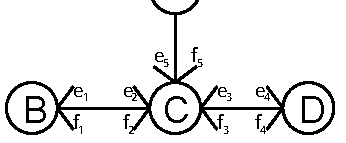
\includegraphics{images/portbondgraph.pdf}
\end{figure}
Conservation of Energy must hold across edges, hence
\[
e_1f_1 +e_2f_2 = 0 \qquad e_3f_3 +e_4f_4 = 0
\]}
\only<2>{
\begin{figure}
	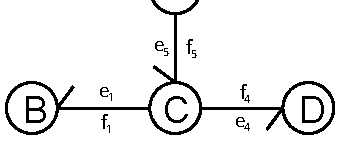
\includegraphics{images/portbondgrapha.pdf}
\end{figure}
We choose a sign, and denote the direction of positive $f$ by a half-arrow.
Hence
\[
e_2 = e_1 \quad f_2 = -f_1 \qquad e_3 = e_4 \quad f_3 = -f_4
\]
which are used to update the co-ordinates of $\Phi_B,\Phi_C$ and $\Phi_D$.
}
\only<3>{
	\begin{figure}
		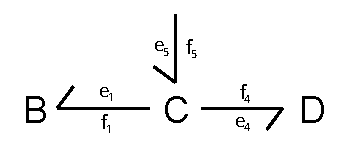
\includegraphics{images/bondgraph.pdf}
	\end{figure}
Discard the extra circles, we get an acasual bond graph.}
\end{frame}
\section{Summary}
\begin{frame}
\frametitle{Acausal Bond Graphs}
	\begin{figure}
	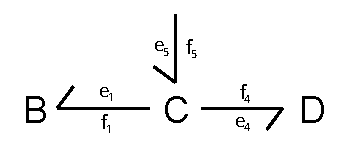
\includegraphics{images/bondgraph.pdf}
\end{figure}
Hence:
\begin{itemize}
	\item A Bond Graph models a network of energetic systems.
	\item A Bond Graph model is not tied to any particular domain.
	\item A Bond Graph is physical so long as the subsystem models $\Phi$ are physical.
\end{itemize}
\emph{These properties make it useful as a general purpose physical modelling language.}
\end{frame}
\begin{frame}
\frametitle{Strengths and Weaknesses}
Strengths:
\begin{itemize}
	\item Cross domain modelling
	\item Modular systems modelling and design that obeys thermodynamics.
	\item Designed to be 'easy' to get equations out the other end. (More on this later)	
\end{itemize}
Weaknesses:
\begin{itemize}
	\item Same as the DSL/GPL tradeoffs in programming.
	\item Requires a different mindset.
	\item Lack of software.
\end{itemize}
\end{frame}

\begin{frame}
\frametitle{Next Time:}
Bond Graph Components\cite{Gaw2015}
\begin{figure}
	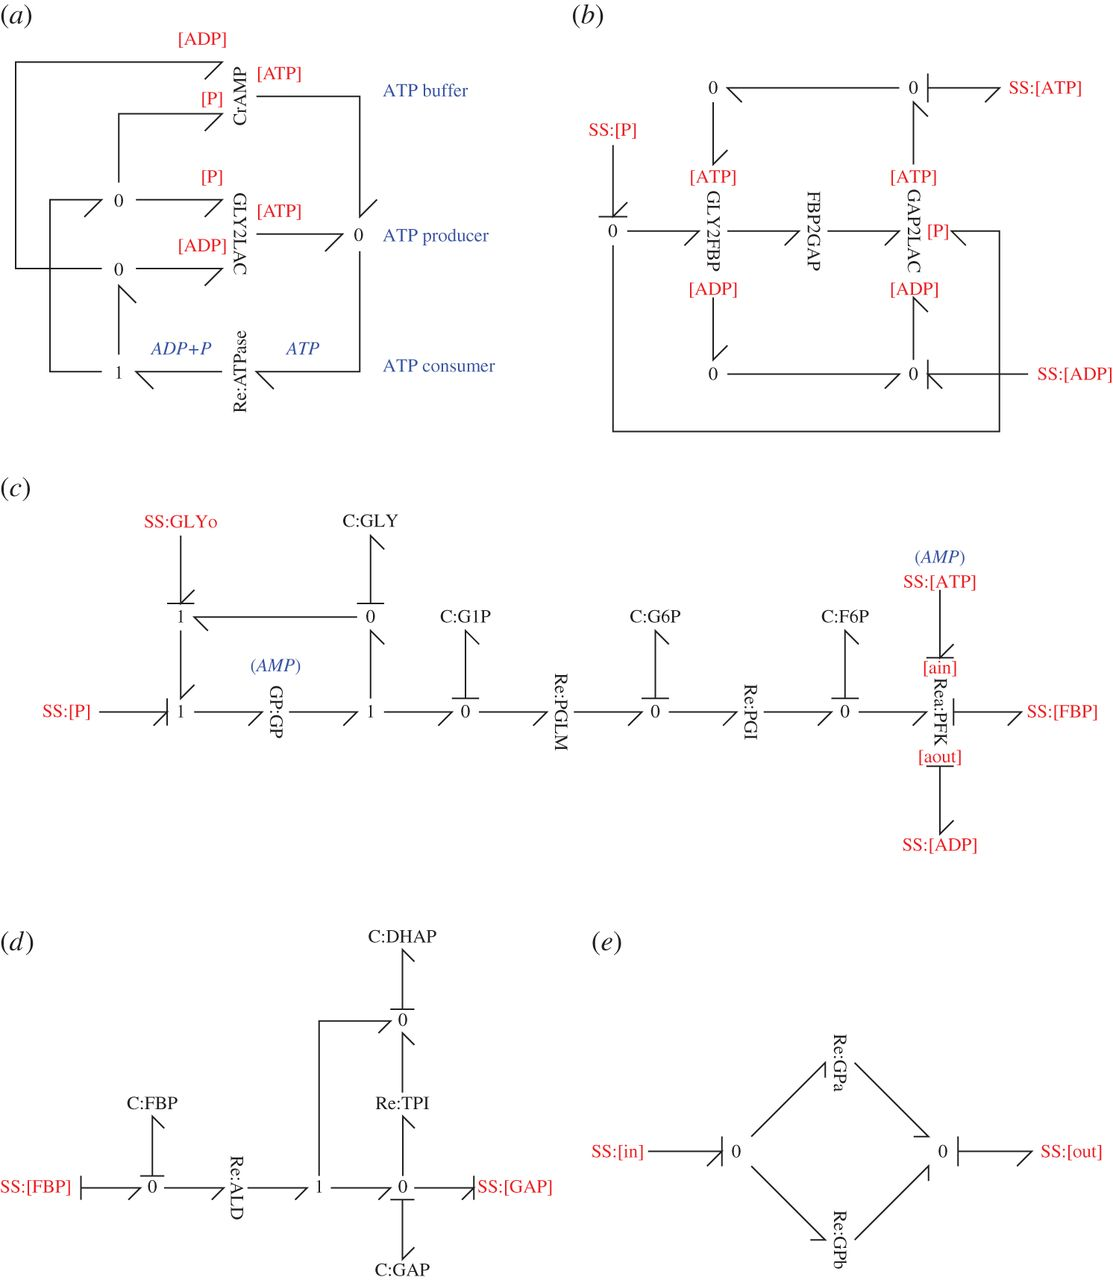
\includegraphics[scale=0.5]{images/F5large.jpg}
\end{figure}


\end{frame}
\begin{thebibliography}{5}
\bibitem{Tran2009} A metabolite-sensitive, thermodynamically-constrained model of cardiac cross-bridge cycling: Implications for force development during ischemia, Kenneth Tran, Nicolas P. Smith, Denis S. Loiselle and Edmund J. Crampin, 2009, \emph{Biophysical Journal}, 98, 267-276
\bibitem{Feynman1961} Feynman, Richard. The Feynman Lectures on Physics; Volume 1. 1964. U.S.A: Addison Wesley. ISBN 0-201-02115-3.
\bibitem{gaw96} Gawthrop, Peter, Smith, Lorcan. Metamodelling: Bond Graphs and Dynamic Systems. 1996.,  Prentice Hall. Hertfordshire UK.
 0-13-489824-9
 \bibitem{Gaw2015}
 Hierarchical bond graph modelling of biochemical networks
 Peter J. Gawthrop, Joseph Cursons, Edmund J. Crampin
 \emph{Proc. R. Soc. A} 2015 471 20150642; DOI: 10.1098/rspa.2015.0642. Published 2 December 2015
 \bibitem{payter2000} http://www.me.utexas.edu/\~longoria/paynter/hmp/Bondgraphs.html
 \bibitem{baez} http://math.ucr.edu/home/baez/week289.html
 \end{thebibliography}
\end{document}